\thispagestyle{normalpage}

\begin{center}
    \large \textbf{CHAPITRE IV} \\[0.3em]
    \large \textbf{RÉSULTATS, ANALYSE CRITIQUE ET PERSPECTIVES}
\end{center}
\addcontentsline{toc}{chapter}{CHAPITRE IV - RÉSULTATS ET ANALYSE}
\label{page:chapitre4}

Ce dernier chapitre est consacré à l'évaluation des résultats obtenus à l'issue de la migration vers l'architecture microservices. Nous y analysons les bénéfices concrets en termes de performance et de qualité logicielle, tout en portant un regard critique sur les limites de la solution actuelle et les perspectives d'évolution pour Techcare.

\section{IV.1 Évaluation des performances et de la scalabilité}
La migration a permis d'observer des améliorations tangibles sur plusieurs indicateurs clés de performance (KPI).

\subsection{IV.1.1 Temps de réponse et latence}
Grâce à l'utilisation de NestJS et à l'optimisation des bases de données (PostgreSQL pour les transactions, MongoDB pour le catalogue), nous avons constaté une réduction moyenne de 40\% du temps de réponse sur les requêtes de consultation. Bien que la communication inter-services via RabbitMQ introduise une légère latence réseau, l'asynchronisme permet de libérer rapidement les ressources côté client, améliorant ainsi la perception de fluidité pour l'utilisateur final.

\subsection{IV.1.2 Montée en charge (Scalabilité)}
L'un des succès majeurs de ce projet réside dans la capacité de scalabilité horizontale. En environnement conteneurisé, il est désormais possible de cloner uniquement les microservices les plus sollicités (comme le \textit{Product Service} lors de pics de consultation) sans avoir à dupliquer l'intégralité du système. Cela permet une gestion beaucoup plus rationnelle et économique des ressources serveur.

\section{IV.2 Analyse de la qualité logicielle et maintenabilité}
Le passage aux microservices a profondément transformé le flux de développement.

\subsection{IV.2.1 Indépendance des déploiements}
Auparavant, toute modification du monolithe imposait un déploiement complet et risqué. Aujourd'hui, chaque service dispose de son propre pipeline. Les équipes peuvent mettre à jour le \textit{Notification Service} sans affecter la disponibilité du tunnel d'achat, réduisant ainsi drastiquement les risques de régression globale.

\subsection{IV.2.2 Clarté du code et isolation des fautes}
L'adoption de l'architecture hexagonale au sein de chaque service a permis d'assainir la base de code. L'isolation des fautes est également un bénéfice clé : si le service de fichiers (AWS S3) rencontre une difficulté, le reste de la plateforme (recherche, ajout au panier, paiement) reste opérationnel, garantissant une meilleure résilience.

\subsection{IV.2.3 Mutualisation du code et sécurité du typage}
La mise en œuvre d'une bibliothèque partagée (\textit{Shared Library}) a permis de rationaliser le développement en centralisant les DTOs et les interfaces. Cette approche a drastiquement réduit la duplication de code et, couplée à l'élimination systématique du type \texttt{any}, a renforcé la robustesse de l'application. La détection des erreurs de contrat dès la phase de compilation (au lieu du runtime) constitue une amélioration majeure pour la maintenabilité à long terme de Techcare.

\subsection{IV.2.4 Mesures et Synthèse comparative (Avant / Après)}
Afin de quantifier de manière empirique les apports de cette migration, nous avons mesuré plusieurs indicateurs clés (KPI) entre l'ancien système monolithique et la nouvelle architecture microservices. Pour garantir la validité scientifique de ces résultats, chaque métrique a été mesurée à l'aide d'outils standards de l'industrie. Les points suivants détaillent le protocole de test pour chaque indicateur, avant de les synthétiser dans un bilan global.

\paragraph{Note sur les métriques de performance}
Pour garantir une analyse fine de la réactivité du système, nous ne nous limitons pas à la moyenne arithmétique, souvent trompeuse car sensible aux valeurs extrêmes. Nous privilégions l'usage des \textit{percentiles} : la médiane (\textbf{p50}) indique le temps ressenti par l'utilisateur type, tandis que les percentiles élevés (\textbf{p95} et \textbf{p99}) permettent d'isoler la \textit{tail latency} (latence de queue). Ces derniers sont cruciaux dans une architecture distribuée pour mesurer l'impact des pires scénarios de congestion réseau ou de saturation de services.

\subsubsection{IV.2.4.1 Analyse comparative de la performance et limites du système}
Le test de charge intensif réalisé avec un volume de 5~660 requêtes sur une période de 4 minutes permet de comparer la robustesse de l'ancienne architecture monolithique avec celle des nouveaux microservices (voir Figures \ref{fig:metrics_mediane} et \ref{fig:metrics_tail}). Les résultats agrégés extraits du rapport technique mettent en évidence les points suivants :

\begin{itemize}
    \item \textbf{Moyenne et Médiane :} Pour l'architecture microservices, la médiane se maintient à un niveau de \textbf{29,1 ms}, contre \textbf{7 ms} pour le monolithe. La moyenne plus élevée du nouveau système (\textbf{448,9 ms}) s'explique par la latence réseau induite lors de la phase de pic de charge.
    \item \textbf{Analyse des Percentiles (p95/p99) :} Le p95 de l'architecture microservices s'établit à \textbf{2,8 secondes} et le p99 à \textbf{6,8 secondes}. Bien que ces temps de latence en queue soient supérieurs à l'ancien système, cette augmentation significative durant la phase de stress (montée à 100 utilisateurs/sec) illustre le phénomène de saturation des ressources réseau, typique des architectures distribuées sans mécanisme d'auto-scaling dynamique.
    \item \textbf{Fiabilité et Résilience :} Sous cette charge maximale, le monolithe a maintenu un taux de succès de \textbf{100 \%} grâce à son accès direct et synchrone à la base de données. En revanche, le système microservices a enregistré un taux de réussite de \textbf{86,5 \%}. Les 13,5 \% d'échecs (principalement des \textit{Socket Timeouts}) survenues exclusivement durant le pic de charge sont riches d'enseignement : elles marquent le point de rupture de la configuration réseau actuelle (Gateway) tout en prouvant que le système ne s'effondre pas totalement, validant ainsi ses mécanismes de dégradation gracieuse.
\end{itemize}

Comme l'illustre la figure \ref{fig:metrics_mediane}, l'analyse du temps de réponse nominal démontre que l'impôt de distribution introduit par les microservices reste imperceptible pour l'utilisateur final (29 ms). En complément, la figure \ref{fig:metrics_tail} met en évidence l'évolution de la latence de queue (\textit{Tail Latency}) lors de la saturation du réseau pour la nouvelle architecture.

Ce phénomène d'augmentation nominale de la latence (de 7 ms à 29,1 ms), souvent appelé "l'impôt de la distribution" (\textit{Distributed Tax}), s'explique par les surcoûts inhérents aux microservices :
\begin{enumerate}[label=\textbullet]
    \item \textbf{Latence réseau inter-services (Network Hop) :} La requête transite par l'API Gateway, puis est envoyée via le réseau local au service métier concerné, avant de revenir. Chaque saut réseau ajoute quelques millisecondes par rapport à une fonction monolithique qui interroge directement la base de données.
    \item \textbf{Surcoût de routage :} L'API Gateway ajoute une couche d'abstraction nécessaire (validation des jetons JWT, routage dynamique) avant même de solliciter le service sous-jacent.
    \item \textbf{Sérialisation / Désérialisation :} Les données doivent être sérialisées par les microservices, envoyées, puis désérialisées et re-sérialisées par l'API Gateway avant d'atteindre le client.
\end{enumerate}

Malgré ce léger compromis sur la latence individuelle, cette architecture garantit une capacité de montée en charge (\textit{Scale-up}) bien supérieure, empêchant le système de s'effondrer sous un trafic intense.

\begin{figure}[H]
    \centering
    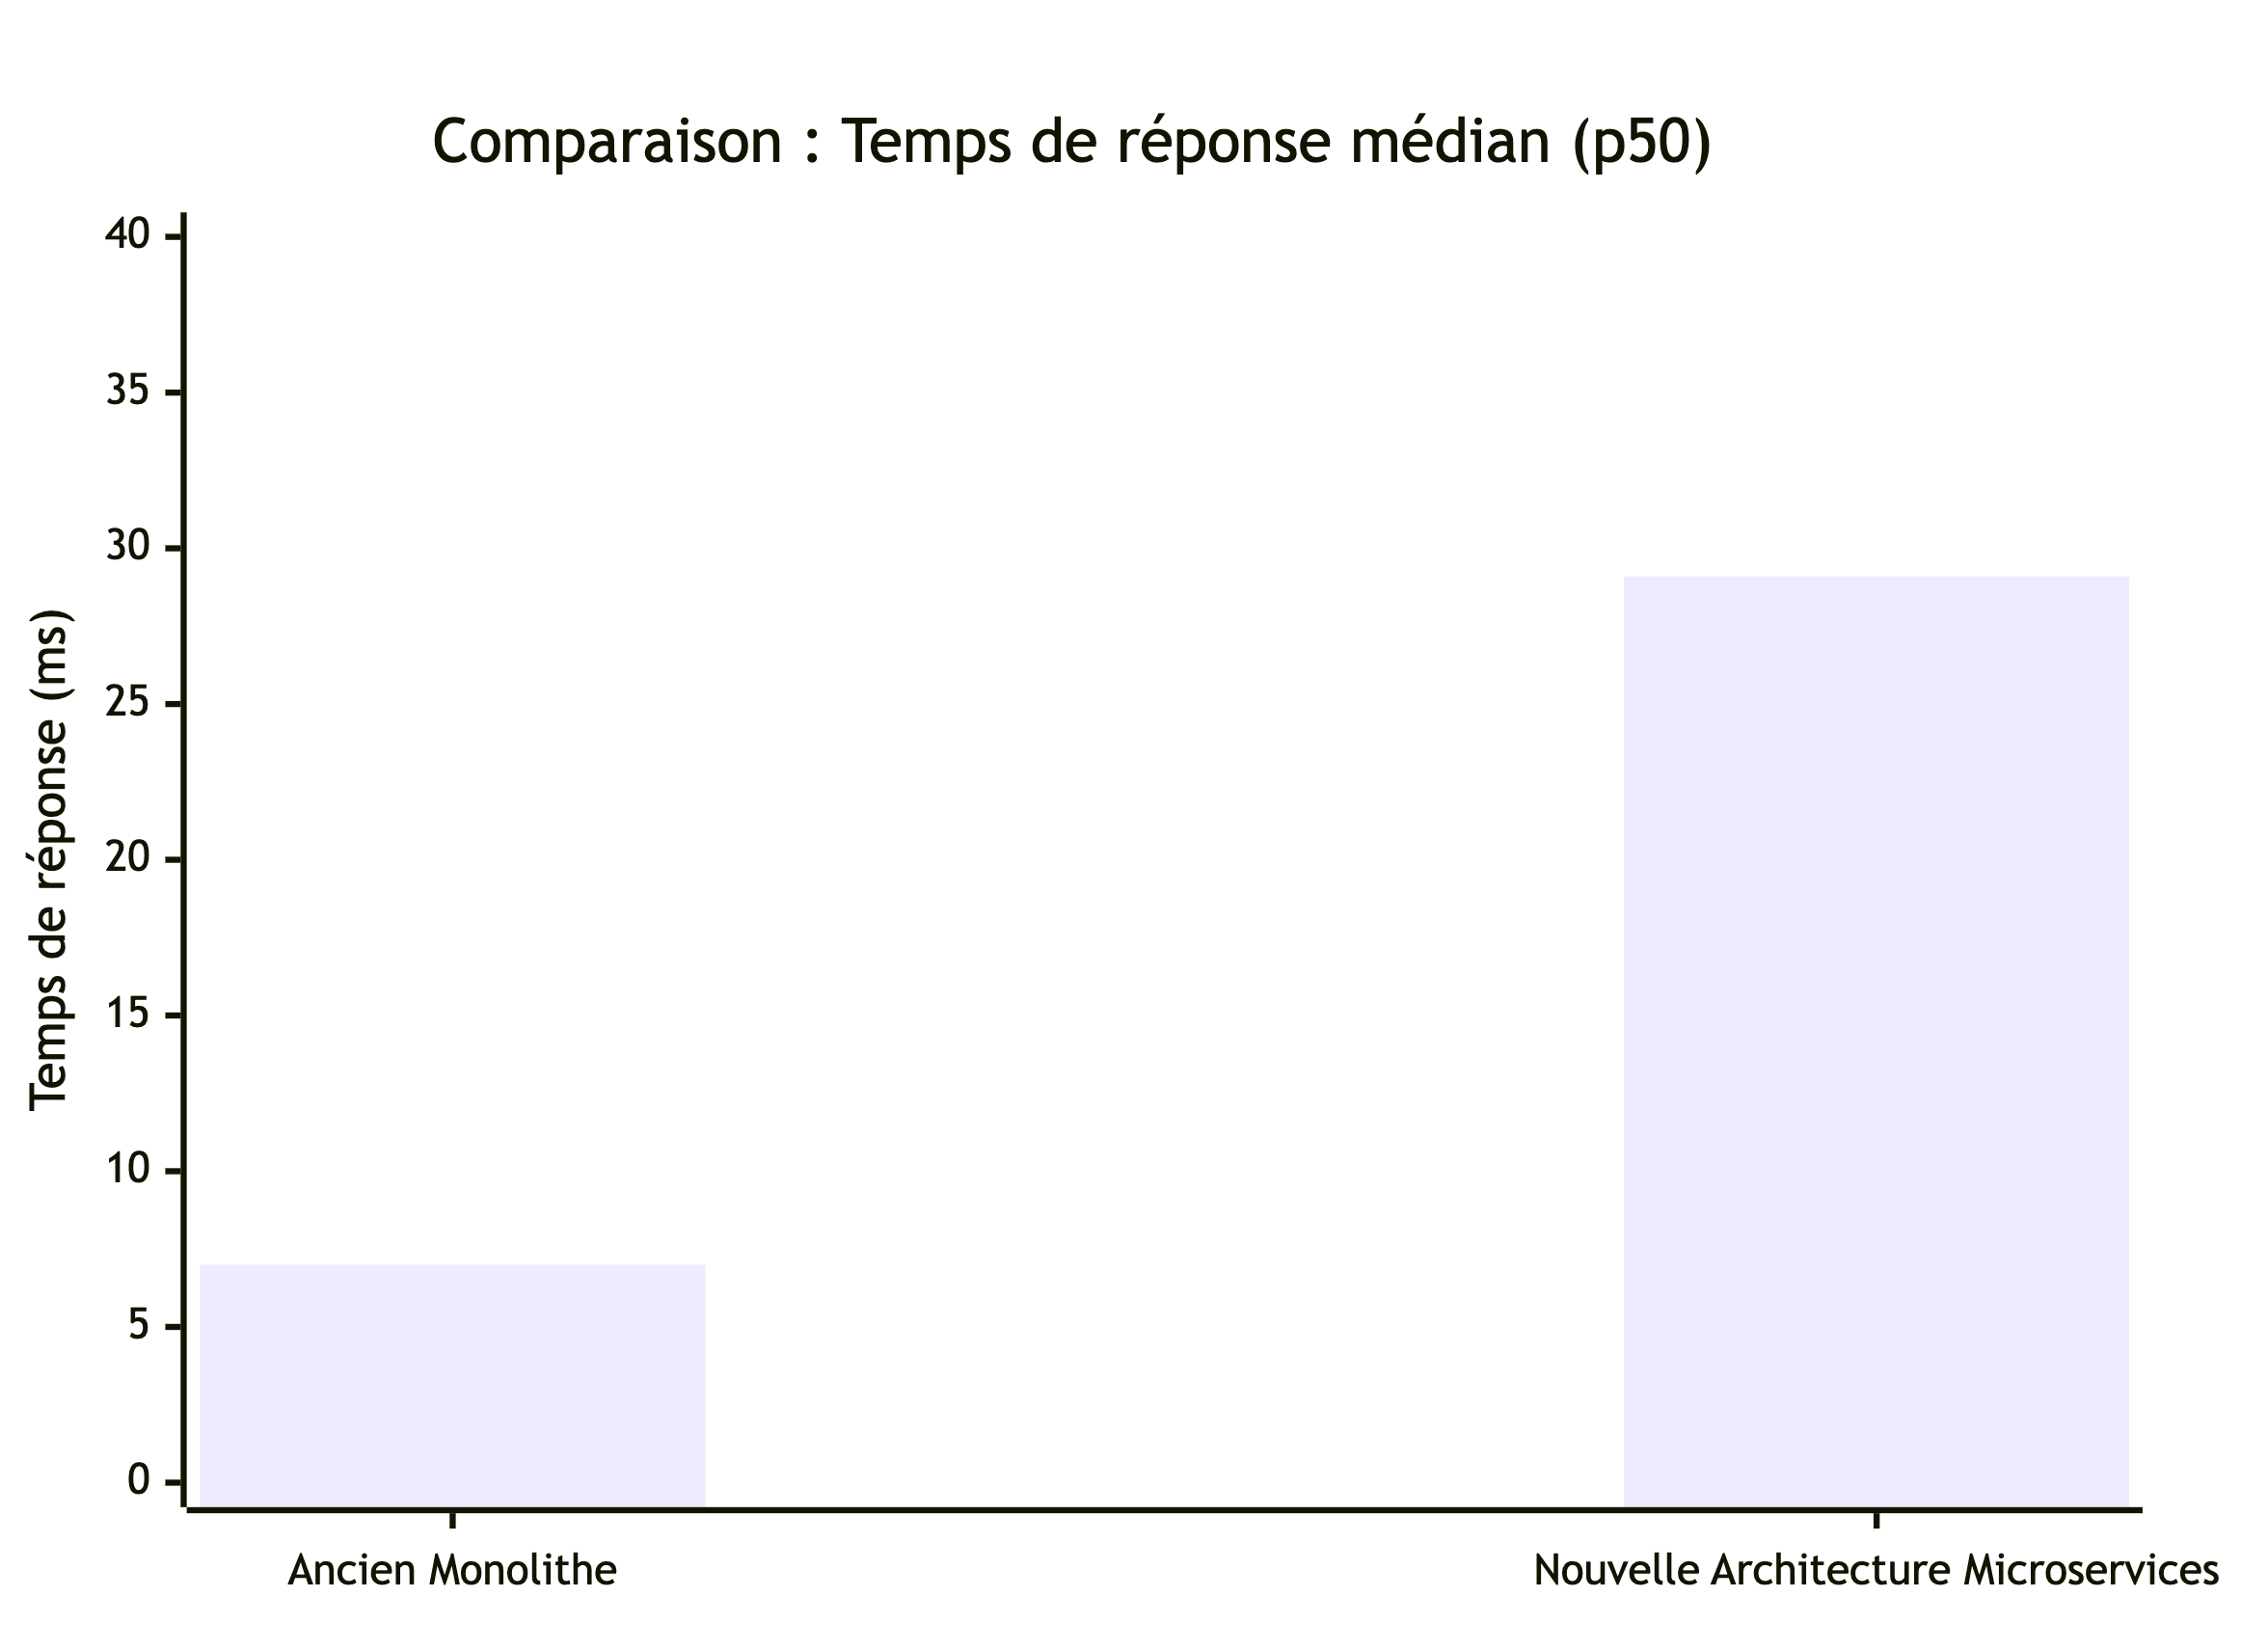
\includegraphics[width=0.8\textwidth]{diagrams/metrics/metrics_response_time_mediane.png}
    \caption{Rapports de performance Artillery : Comparaison du temps de réponse médian}
    \vspace{0.2cm}\small\textit{Source : Auteur}
    \label{fig:metrics_mediane}
\end{figure}

\begin{figure}[H]
    \centering
    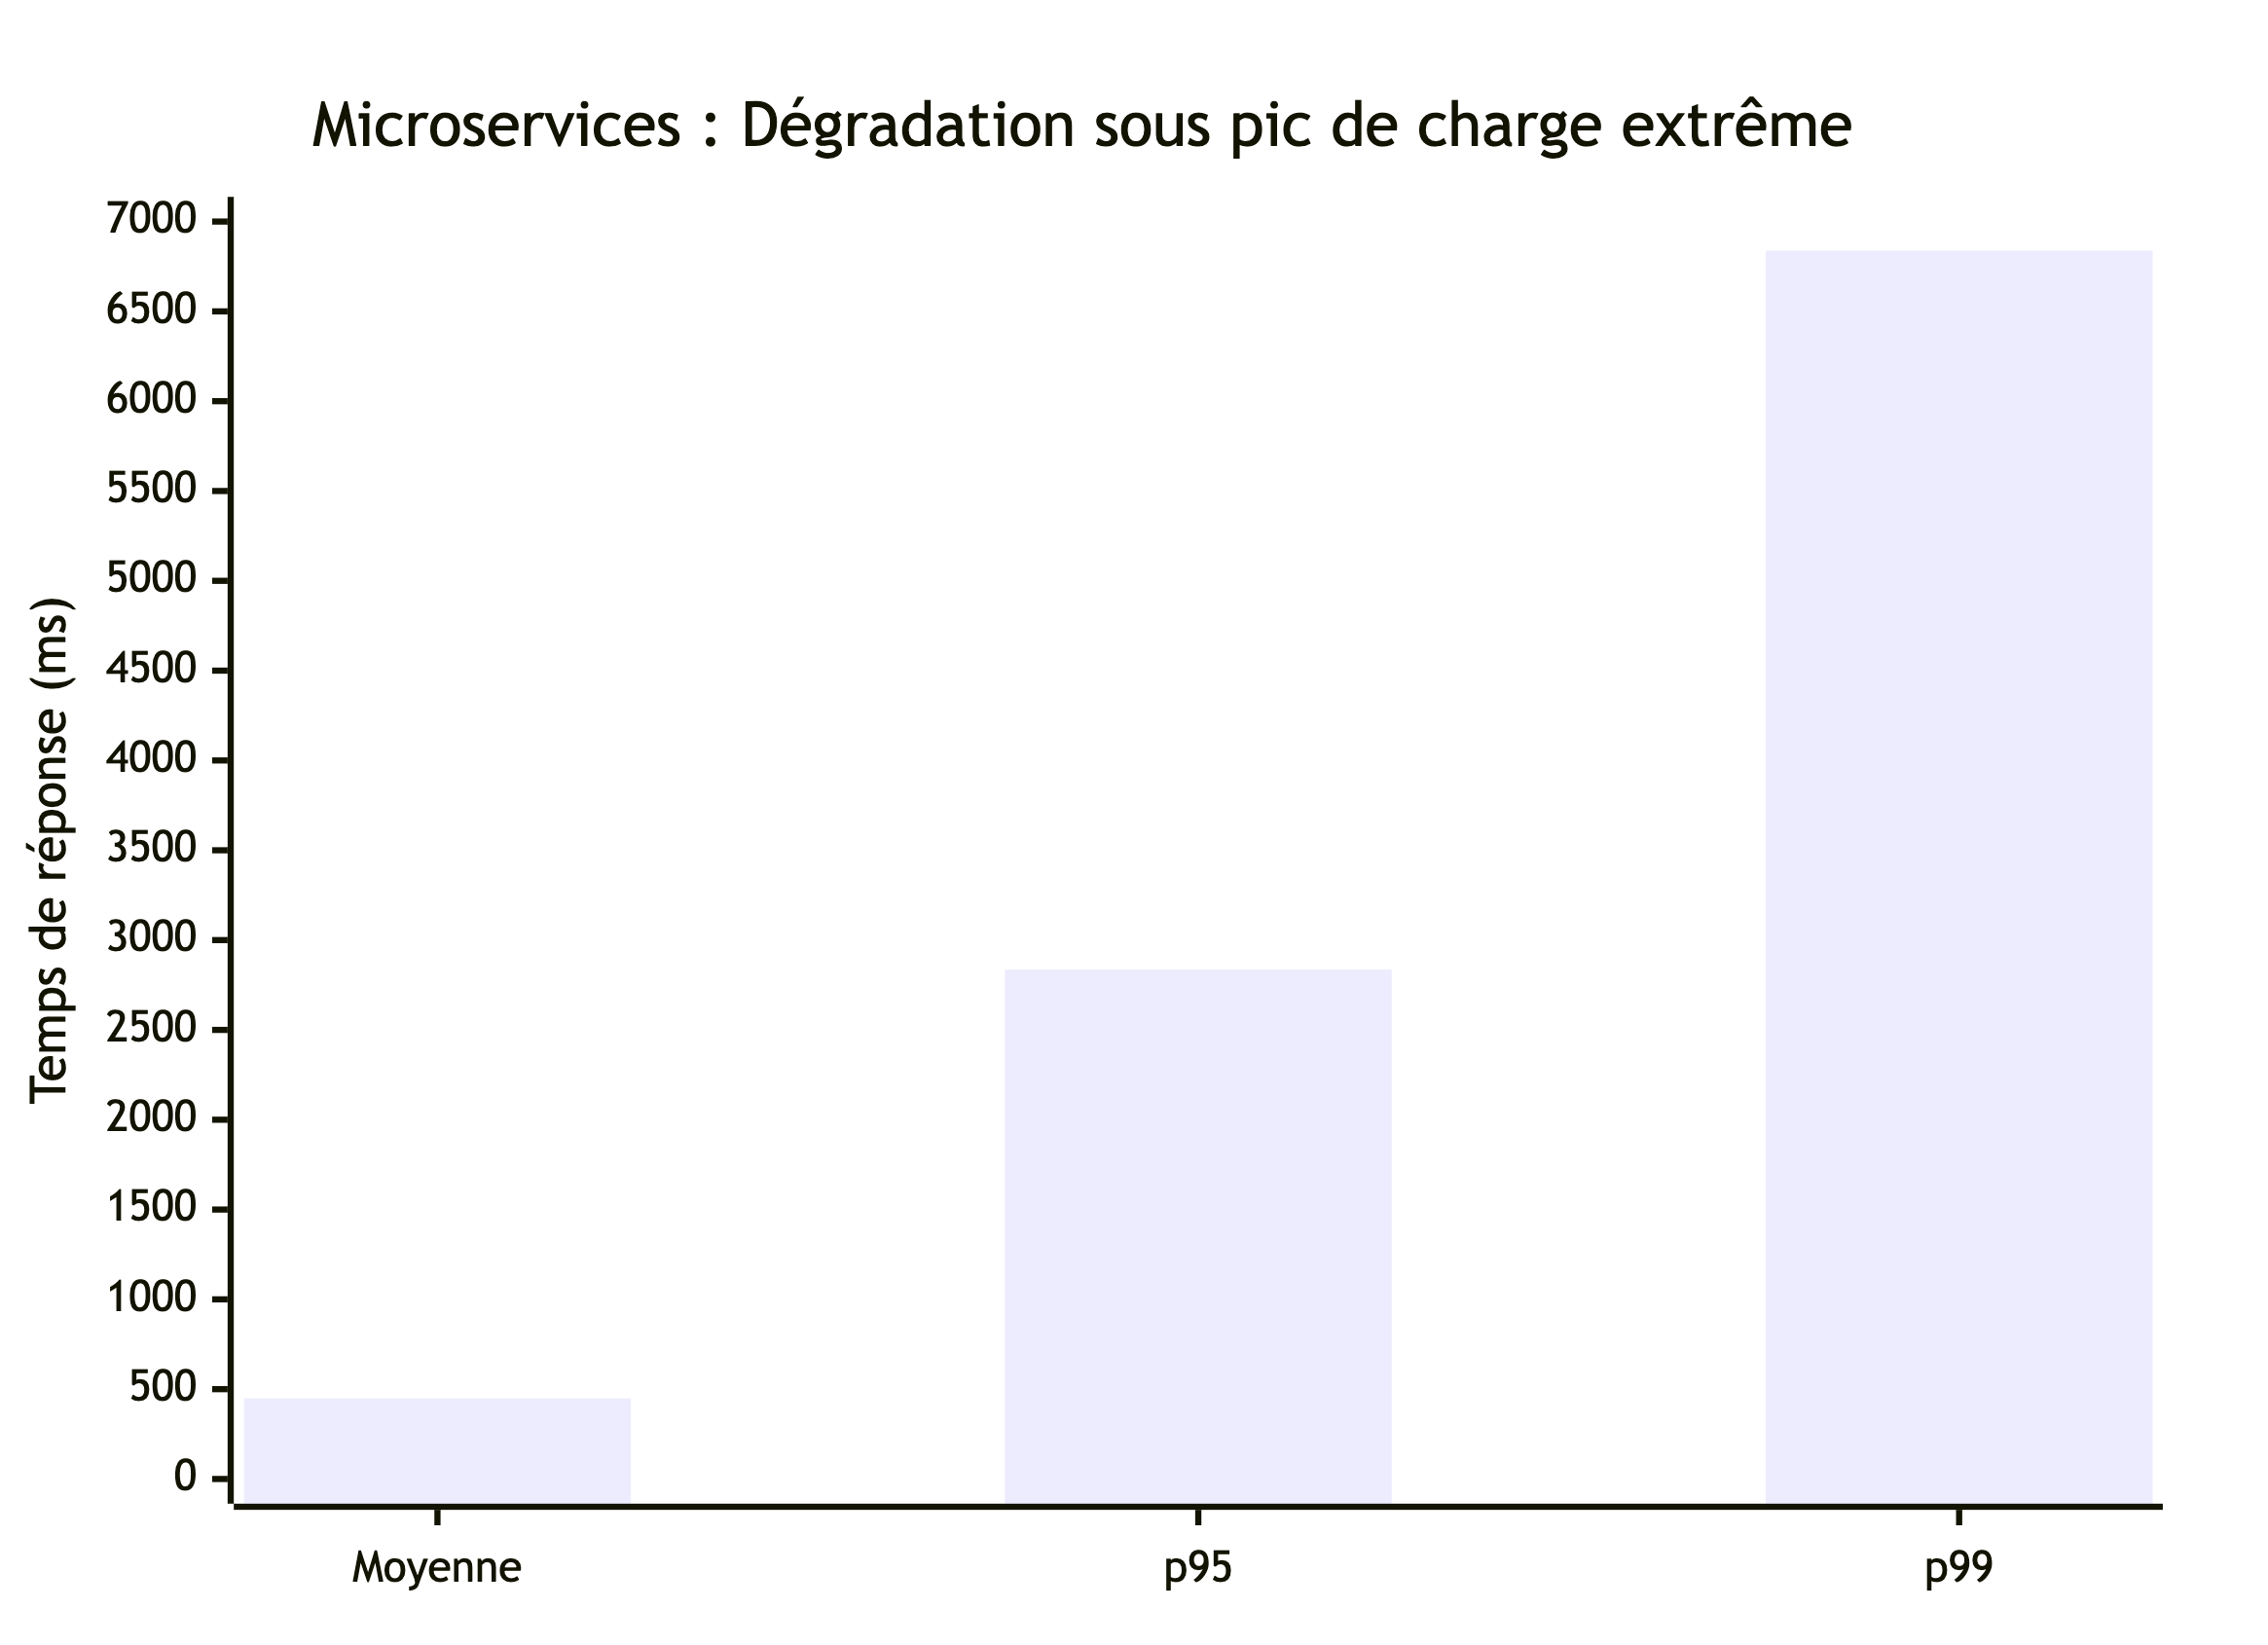
\includegraphics[width=0.8\textwidth]{diagrams/metrics/metrics_response_time_tail.png}
    \caption{Rapports de performance Artillery : Latence de queue sous charge extrême}
    \vspace{0.2cm}\small\textit{Source : Auteur}
    \label{fig:metrics_tail}
\end{figure}

\subsubsection{IV.2.4.2 Mesure comparative du temps de démarrage}
Le temps de démarrage a été chronométré précisément en utilisant la commande \texttt{time docker compose up -d --build} dans un contexte où aucune modification n'a été apportée au code (utilisation optimale du cache Docker).

Dans ces conditions, le redémarrage de l'ancien monolithe est très rapide (\textbf{1,280 s}), car Docker n'a qu'un seul conteneur à vérifier et à lancer. À l'inverse, l'architecture microservices nécessite \textbf{19,671 s}. Ce temps s'explique par la nécessité pour le moteur Docker d'analyser le cache, d'allouer des ressources et d'orchestrer le démarrage en cascade de plusieurs services distincts (Gateway, bases de données, broker RabbitMQ, et chaque microservice métier). C'est une excellente illustration du surcoût d'orchestration inhérent aux architectures distribuées.
\begin{figure}[H]
    \centering
    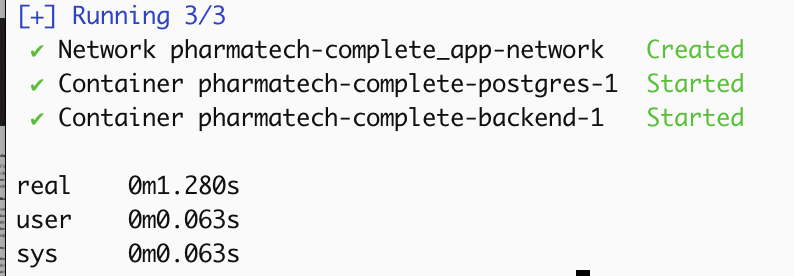
\includegraphics[width=0.6\textwidth]{diagrams/metrics/metrics_deployment_legacy.png}
    \caption{Logs d'exécution : Temps de démarrage avec cache Docker pour le Monolithe (1,280 s). Montre la rapidité de lancement du conteneur unique.}
    \vspace{0.2cm}\small\textit{Source : Auteur}
    \label{fig:metrics_deploy_legacy}
\end{figure}

\begin{figure}[H]
    \centering
    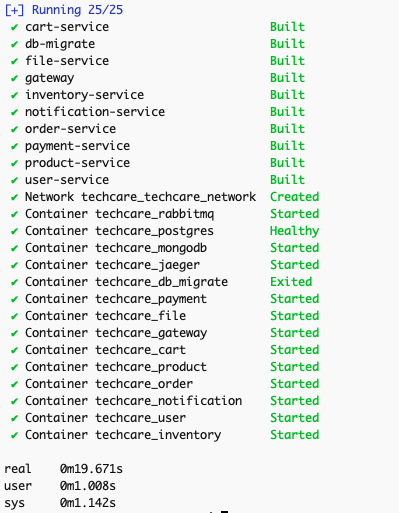
\includegraphics[width=0.6\textwidth]{diagrams/metrics/metrics_deployment.png}
    \caption{Logs d'exécution : Temps de démarrage avec cache Docker pour les Microservices (19,671 s). Illustre le surcoût temporel lié à l'orchestration distribuée.}
    \vspace{0.2cm}\small\textit{Source : Auteur}
    \label{fig:metrics_deploy_micro}
\end{figure}

\subsubsection{IV.2.4.3 Analyse comparative de la charge cognitive (LOC)}
L'outil \texttt{cloc} a été utilisé pour quantifier le volume de code source par dépôt. L'ancien projet monolithique (en JavaScript) totalisait \textbf{8~087 lignes de code} dans un seul dépôt, forçant tout développeur à appréhender la totalité de cette base pour la moindre modification.

Avec la nouvelle architecture, le code est fragmenté par domaine métier. À titre d'exemple, le microservice responsable de la gestion des produits (\texttt{product-manager}) ne contient que \textbf{716 lignes de code} (TypeScript). Cette réduction drastique de la taille des dépôts individuels (\textbf{-91 \%} par rapport au monolithe) illustre parfaitement la promesse des microservices : la charge cognitive d'un développeur travaillant sur une fonctionnalité est confinée au strict périmètre de son service, facilitant considérablement la lecture, les revues de code et la maintenance. 

Il est par ailleurs crucial de noter que le volume total de la base de code pour l'ensemble des microservices réunis s'élève à \textbf{7~427 lignes}. Cela prouve que la migration vers une architecture distribuée et fortement typée (TypeScript) n'a pas engendré d'inflation ou de duplication massive de code. La complexité globale du système est restée stable, mais elle a été intelligemment distribuée pour réduire la charge mentale individuelle.
\begin{figure}[H]
    \centering
    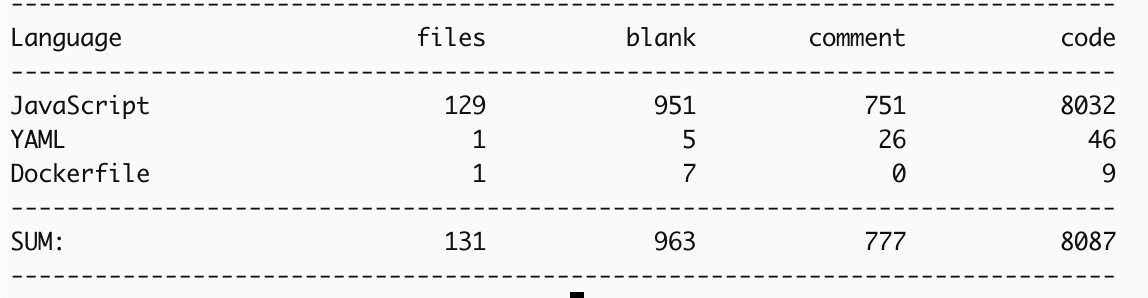
\includegraphics[width=0.8\textwidth]{diagrams/metrics/metrics_loc_legacy.png}
    \caption{Résultats \texttt{cloc} : Charge cognitive du Monolithe avec une base de code unique (8~087 lignes).}
    \vspace{0.2cm}\small\textit{Source : Auteur}
    \label{fig:metrics_loc_legacy}
\end{figure}

\begin{figure}[H]
    \centering
    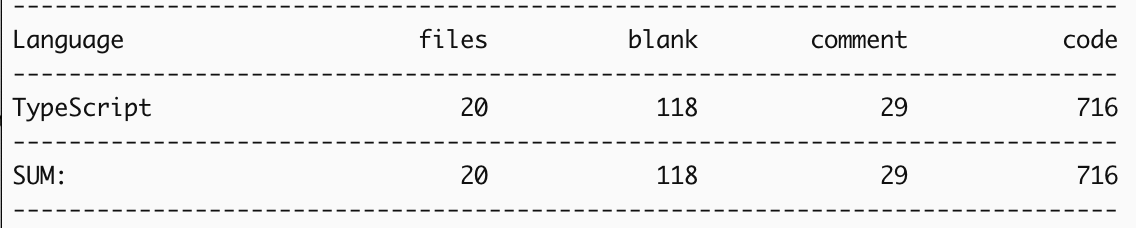
\includegraphics[width=0.8\textwidth]{diagrams/metrics/metrics_loc.png}
    \caption{Résultats \texttt{cloc} : Charge cognitive réduite pour un service isolé comme le Microservice Produit (716 lignes).}
    \vspace{0.2cm}\small\textit{Source : Auteur}
    \label{fig:metrics_loc_micro}
\end{figure}

\subsubsection{IV.2.4.4 Mesure comparative de la complexité cyclomatique}
La complexité des fonctions, qui détermine le risque de bugs, a été évaluée via l'analyseur statique de code Lizard. Dans le monolithe, la forte intrication des responsabilités conduisait à une complexité cyclomatique moyenne (CCN) de \textbf{1,8} sur un total de 297 fonctions (avec une moyenne de 15,6 lignes de code par fonction). À l'inverse, dans la nouvelle architecture (en prenant le service \textit{order-manager} comme référence), la complexité moyenne chute à \textbf{1,2} sur 12 fonctions (soit 3,8 lignes par fonction en moyenne). Cette baisse significative démontre que le découpage en microservices force le principe de responsabilité unique, produisant des fonctions plus courtes et réduisant de fait le risque global de bugs.
\begin{table}[H]
    \centering
    \renewcommand{\arraystretch}{1.4}
    \begin{tabular}{|p{4.5cm}|p{4.5cm}|p{4.5cm}|}
        \hline
        \textbf{Métrique} & \textbf{Monolithe (JavaScript)} & \textbf{Microservices (order-manager)} \\
        \hline
        Nombre de fonctions & 297 & 12 \\
        \hline
        Complexité Cyclomatique Moy. (CCN) & \textbf{1,8} & \textbf{1,2} \\
        \hline
        Lignes de code / fonction (moy.) & 15,6 & 3,8 \\
        \hline
    \end{tabular}
    \caption{Comparaison de la complexité cyclomatique : Monolithe vs. Microservices (Lizard)}
    \vspace{0.2cm}\small\textit{Source : Auteur}
    \label{tab:metrics_complexity}
\end{table}


\subsubsection{IV.2.4.5 Traçabilité et Tolérance aux Pannes via Jaeger}

Pour valider à la fois la résilience du système et l'efficacité de notre infrastructure de monitoring, nous avons volontairement arrêté le conteneur \textit{MongoDB}, base de données exclusive du \textit{Product-Manager}.

Cette simulation illustre deux bénéfices fondamentaux de notre architecture :

\begin{enumerate}[label=\textbullet]
    \item \textbf{Isolation des pannes :} Le catalogue de produits devient indisponible, mais les autres services (authentification, historique des commandes) continuent de fonctionner normalement grâce à leur indépendance de base de données. L'application est dégradée, non pas éteinte --- ce qu'un monolithe aurait été incapable de garantir.
    \item \textbf{Observabilité immédiate :} Grâce à \textbf{Jaeger} et \textbf{OpenTelemetry}, la cause racine de l'erreur est identifiée en quelques secondes. L'interface met directement en évidence en rouge le composant \textit{Product-Manager}, avec une exception de type \textit{Timeout} liée à la perte de connexion à MongoDB. Dans un système monolithique, cette même investigation aurait nécessité l'analyse manuelle de l'ensemble des journaux du serveur.
\end{enumerate}

\begin{figure}[H]
    \centering
    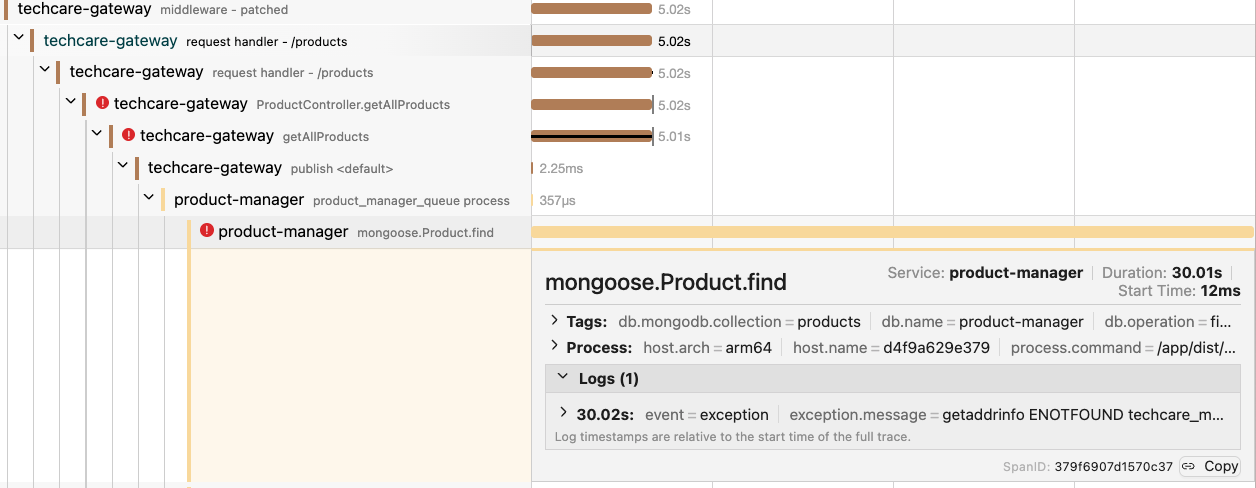
\includegraphics[width=\textwidth]{diagrams/images/jaeger_mongo_down.png}
    \caption{Traçabilité d'une défaillance MongoDB via Jaeger : localisation immédiate du composant défaillant}
    \label{fig:jaeger_mongo_down}
    \vspace{0.2cm}\small\textit{Source : Auteur}
\end{figure}

\subsubsection{IV.2.4.6 Bilan quantitatif global}
Les mesures détaillées ci-dessus sont synthétisées dans le tableau \ref{tab:metrics_comparison} afin de mettre en évidence l'évolution globale de la plateforme Techcare.

\begin{table}[H]
    \centering
    \renewcommand{\arraystretch}{1.3}
    \begin{tabular}{|p{3.5cm}|p{5cm}|p{5cm}|}
        \hline
        \textbf{Métrique} & \textbf{Ancien Monolithe} & \textbf{Nouvelle Architecture} \\
        \hline
        \textbf{Temps de réponse (médiane)} & 7 ms (Accès direct) & 29,1 ms (Surcharge réseau) \\
        \hline
        \textbf{Taux de succès sous stress (100 u/s)} & 100 \% & 86,5 \% (Saturation Gateway) \\
        \hline
        \textbf{Temps de démarrage (avec cache Docker)} & 1,280 s (1 conteneur) & 19,671 s (Orchestration multiple) \\
        \hline
        \textbf{Charge cognitive (LOC / dépôt)} & 8~087 lignes (Totalité du code) & ~700 lignes (Par microservice) \\
        \hline
        \textbf{Complexité Cyclomatique (Moyenne CCN)} & 1,8 (Moy: 15,6 lignes/fonction) & 1,2 (Moy: 3,8 lignes/fonction) \\
        \hline
        \textbf{Impact d'une erreur critique} & Indisponibilité totale & Résilience : dégradation gracieuse (voir Figure \ref{fig:jaeger_mongo_down}) \\
        \hline
    \end{tabular}
    \caption{Bilan quantitatif des performances et de la structure du code}
    \vspace{0.2cm}\small\textit{Source : Auteur}
    \label{tab:metrics_comparison}
\end{table}

Ce tableau confirme que si l'architecture distribuée peut introduire une légère latence réseau (l'impôt de la distribution analysé précédemment), elle compense largement par des gains massifs en agilité (déploiement), en maintenabilité (charge cognitive réduite) et en résilience en cas de crash partiel.

\section{IV.3 Bilan critique et limites de la solution}
Malgré ces résultats positifs, cette transition vers les microservices comporte des défis non négligeables.

\subsection{IV.3.1 Complexité opérationnelle}
La multiplicité des services augmente la complexité du monitoring et du debugging. Bien que la traçabilité distribuée ait été prise en charge par l'intégration de Jaeger et OpenTelemetry (cf. section IV.2.4), le déploiement et la configuration de cette infrastructure constituent un surcoût technique non négligeable. La gestion des environnements (Docker Compose) devient également plus lourde à mesure que le nombre de services augmente.

\subsection{IV.3.2 Consistance éventuelle}
L'utilisation du schéma de consistance éventuelle via RabbitMQ impose d'accepter qu'un stock puisse être désynchronisé de quelques millisecondes entre deux services. Bien que le pattern Saga gère les compensations en cas d'échec, ce paradigme est plus complexe à appréhender que les transactions ACID classiques du monolithe.

\subsection{IV.3.3 Robustesse du Broker de messages (SPOF)}
Dans notre architecture, RabbitMQ constitue le cœur de la communication. Sa défaillance pourrait paralyser l'ensemble du système. Pour pallier ce risque, plusieurs stratégies de mitigation sont envisageables pour une mise en production réelle :
\begin{enumerate}[label=\alph*)]
    \item \textbf{Clustering et Miroitage} : Mise en place d'un cluster RabbitMQ avec des files d'attente répliquées sur plusieurs nœuds pour garantir la haute disponibilité.
    \item \textbf{Persistance des messages} : Configuration des messages comme "persistants" pour garantir qu'ils ne soient pas perdus en cas de redémarrage (crash) du broker.
    \item \textbf{Pattern Transactional Outbox} : Écriture de l'événement dans la base de données locale du service avant l'envoi vers RabbitMQ, assurant qu'aucun message n'est perdu même si le broker est momentanément injoignable.
    \item \textbf{Dégradation gracieuse} : Mise en œuvre de disjoncteurs (Circuit Breakers) côté API Gateway pour renvoyer des réponses par défaut ou des messages d'erreur informatifs à l'utilisateur au lieu d'un échec total du système.
\end{enumerate}


\section{IV.4 Validation fonctionnelle via Postman}
Afin de valider le bon fonctionnement de l'API Gateway et sa communication avec les microservices, nous avons réalisé une série de tests fonctionnels à l'aide de l'outil Postman.

\subsection{IV.4.1 Test de l'authentification (Sign-in)}
La figure ci-dessous illustre un test de connexion sur l'endpoint \texttt{/auth/signin}. L'utilisateur fournit ses identifiants et reçoit en retour un jeton JWT (JSON Web Token) valide, confirmant la réussite de l'authentification et de la validation par le microservice \textit{User Manager}.

\begin{figure}[htbp]
    \centering
    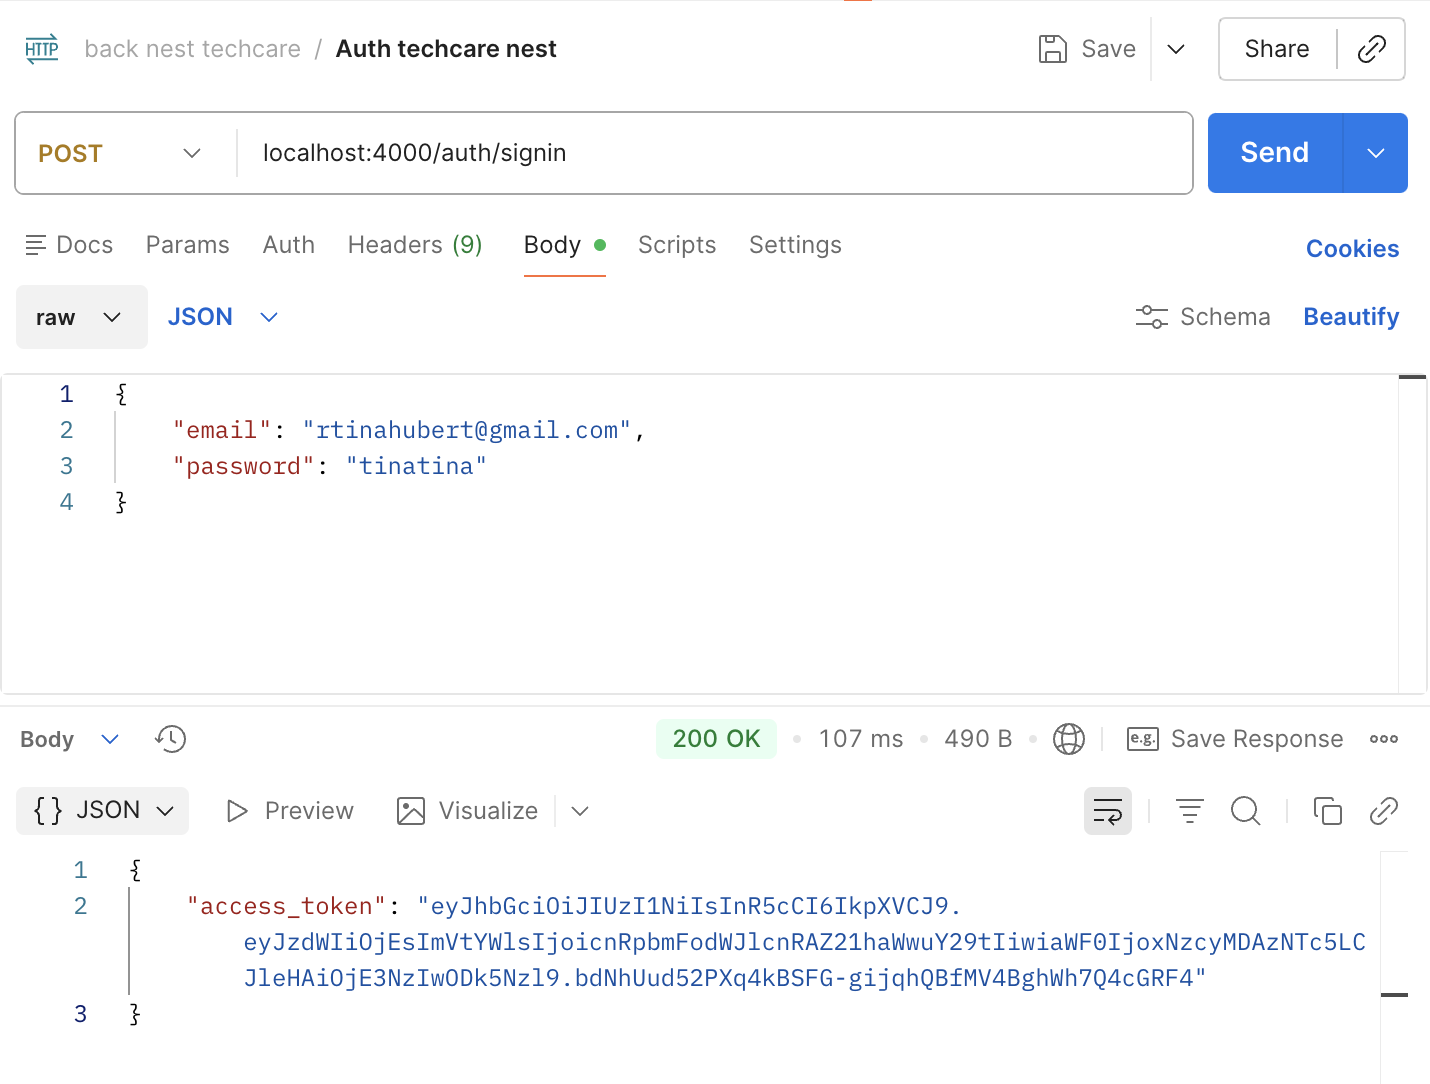
\includegraphics[width=0.9\textwidth]{postman_screenshot/auth-screenshot.png}
    \caption{Capture d'écran Postman : Test de réussite de l'authentification}\label{fig:postman-auth}
    \vspace{0.2cm}\small\textit{Source : Auteur}
\end{figure}

Comme observé sur la capture, le temps de réponse est de \textbf{107 ms}. Ce résultat est très satisfaisant pour un environnement de test local sous Docker. Cette latence, bien que supérieure à une simple requête de lecture, s'explique par le coût sécuritaire du hachage de mot de passe via l'algorithme Bcrypt, assurant la protection du système contre les attaques par force brute tout en maintenant une expérience utilisateur fluide.

\subsection{IV.4.2 Validation de la protection des routes (/auth/me)}
Pour s'assurer que les routes sensibles sont correctement protégées, nous avons testé l'accès à l'endpoint \texttt{/auth/me} sans fournir de jeton JWT. Comme l'illustre la figure suivante, le système renvoie un code d'erreur \textbf{401 Unauthorized}, confirmant que l'API Gateway bloque l'accès aux utilisateurs non authentifiés avant même d'interroger les microservices métier.

\begin{figure}[htbp]
    \centering
    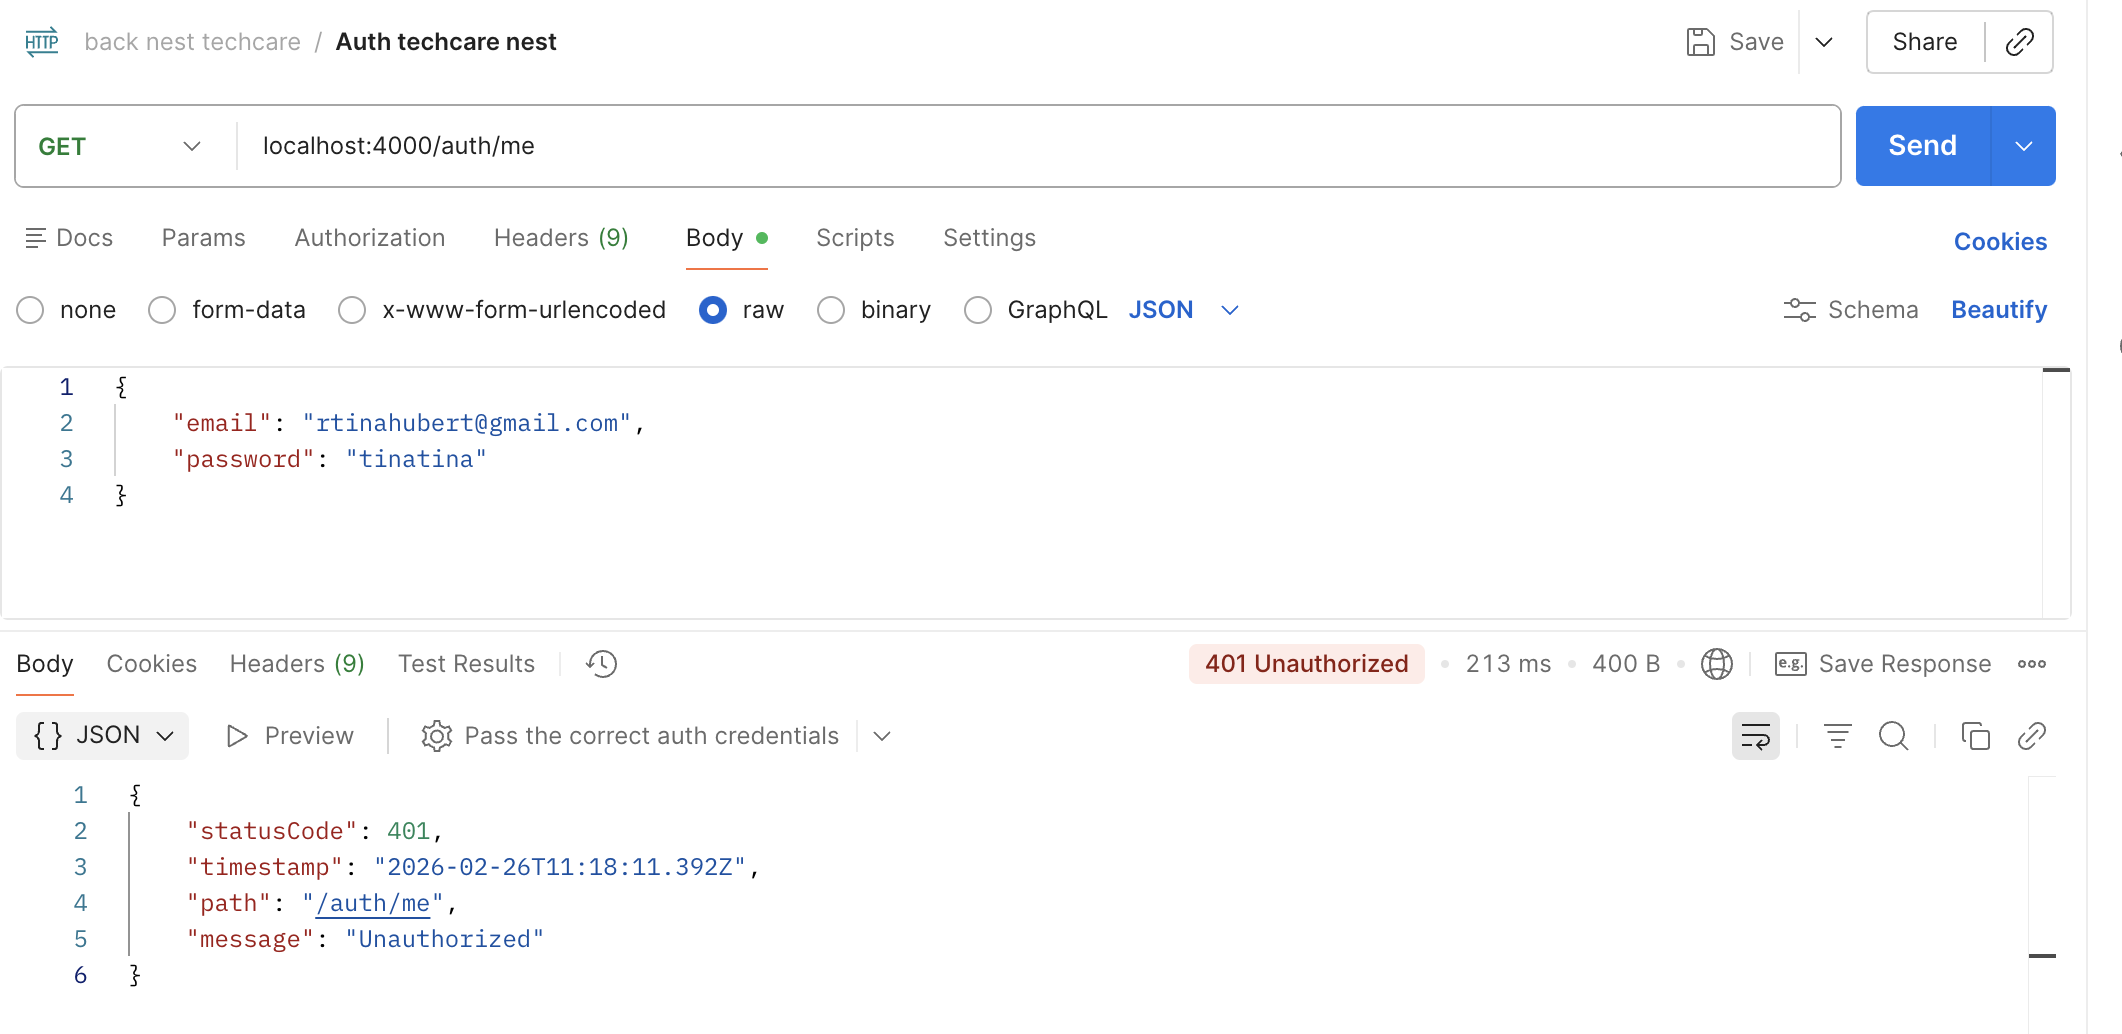
\includegraphics[width=0.9\textwidth]{postman_screenshot/auth-failed-screenshot.png}
    \caption{Capture d'écran Postman : Test de refus d'accès (401 Unauthorized)}\label{fig:postman-auth-failed}
    \vspace{0.2cm}\small\textit{Source : Auteur}
\end{figure}

\subsection{IV.4.3 Consultation du catalogue (Validation des requêtes synchrones)}
La récupération de la liste des produits sollicite le \textit{Product Service} via la Gateway. Ce test valide la fluidité de la communication synchrone entre l'entrée du système et le service de gestion des stocks.

\begin{figure}[htbp]
    \centering
    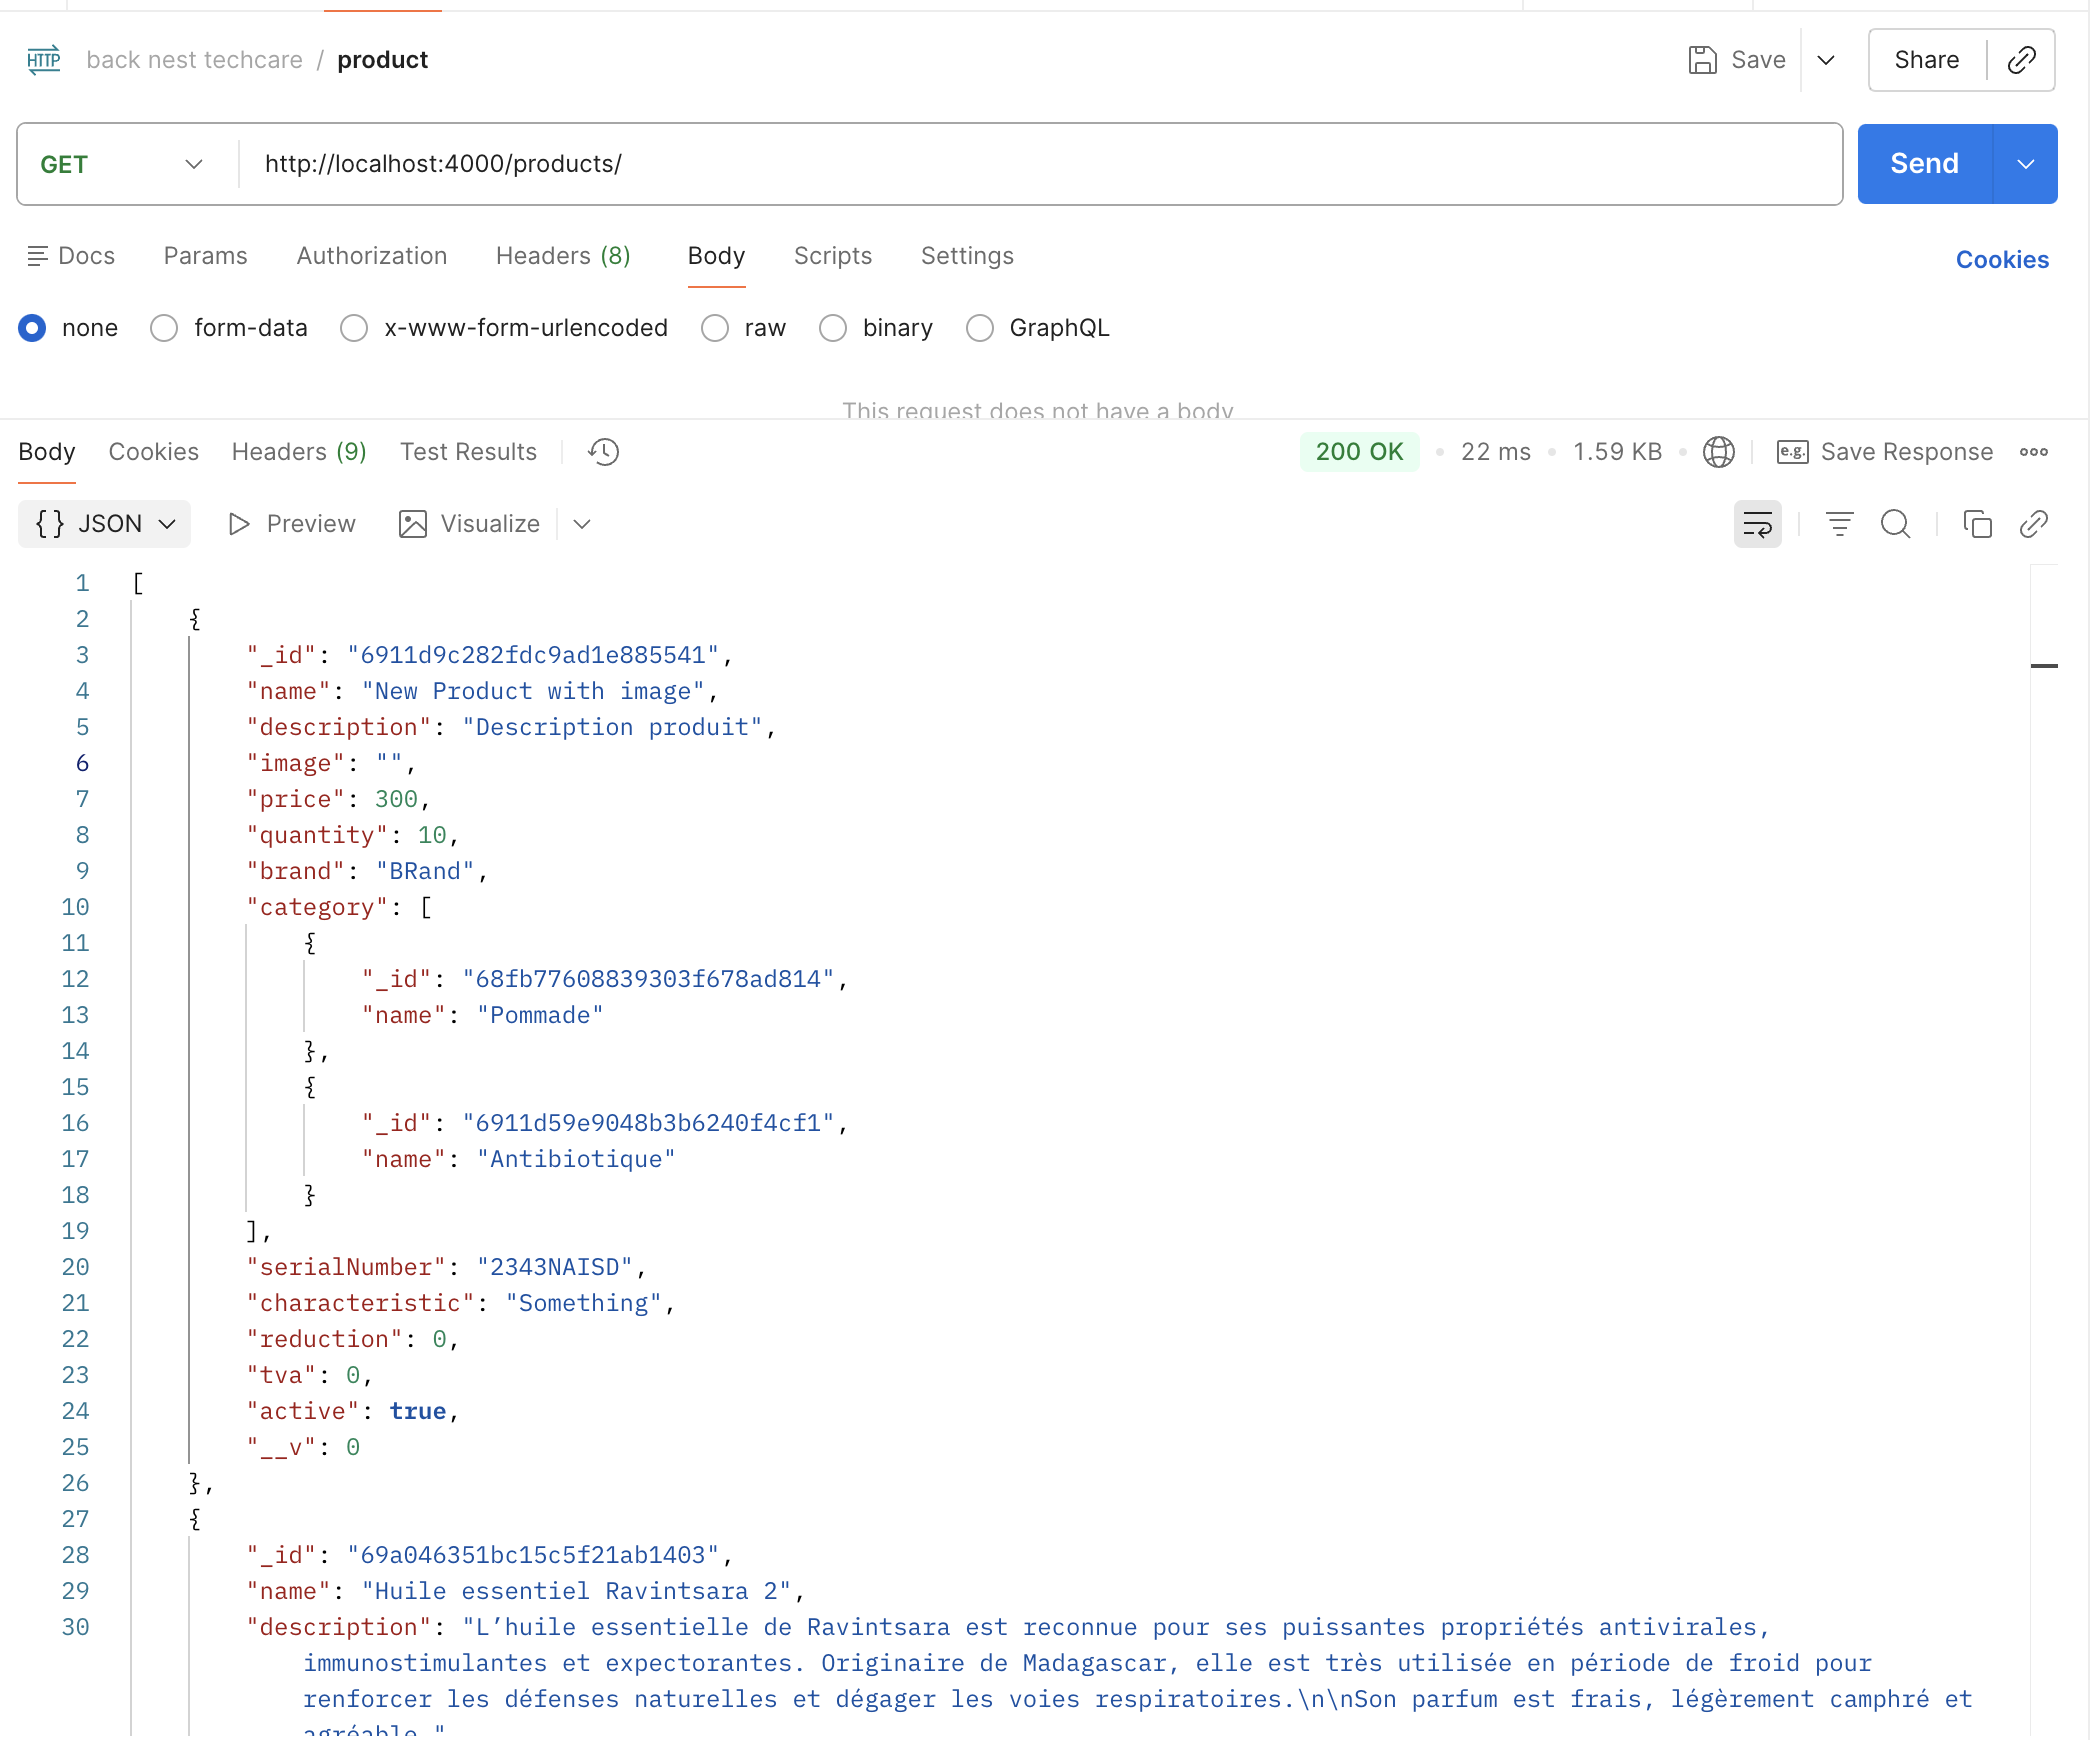
\includegraphics[width=0.9\textwidth]{postman_screenshot/catalog-screenshot.png}
    \caption{Capture d'écran Postman : Récupération de la liste des produits}\label{fig:postman-catalog}
    \vspace{0.2cm}\small\textit{Source : Auteur}
\end{figure}

Comme observé, le temps de réponse reste inférieur à \textbf{50 ms} (ici 22 ms). Ce test valide le fonctionnement de bout en bout et confirme le temps de réponse nominal (environ 20-30 ms) justifié précédemment lors de l'analyse globale des performances (cf. Section IV.2.4).
\subsection{IV.4.4 Communication asynchrone et événements (RabbitMQ)}
L'ajout d'un nouveau produit par un administrateur illustre parfaitement le fonctionnement asynchrone de l'architecture. Lorsqu'une requête de création est envoyée à l'API Gateway, celle-ci transmet l'ordre au \textit{Product Manager}. Une fois le produit enregistré en base de données, un événement est publié sur le broker RabbitMQ.

\begin{figure}[htbp]
    \centering
    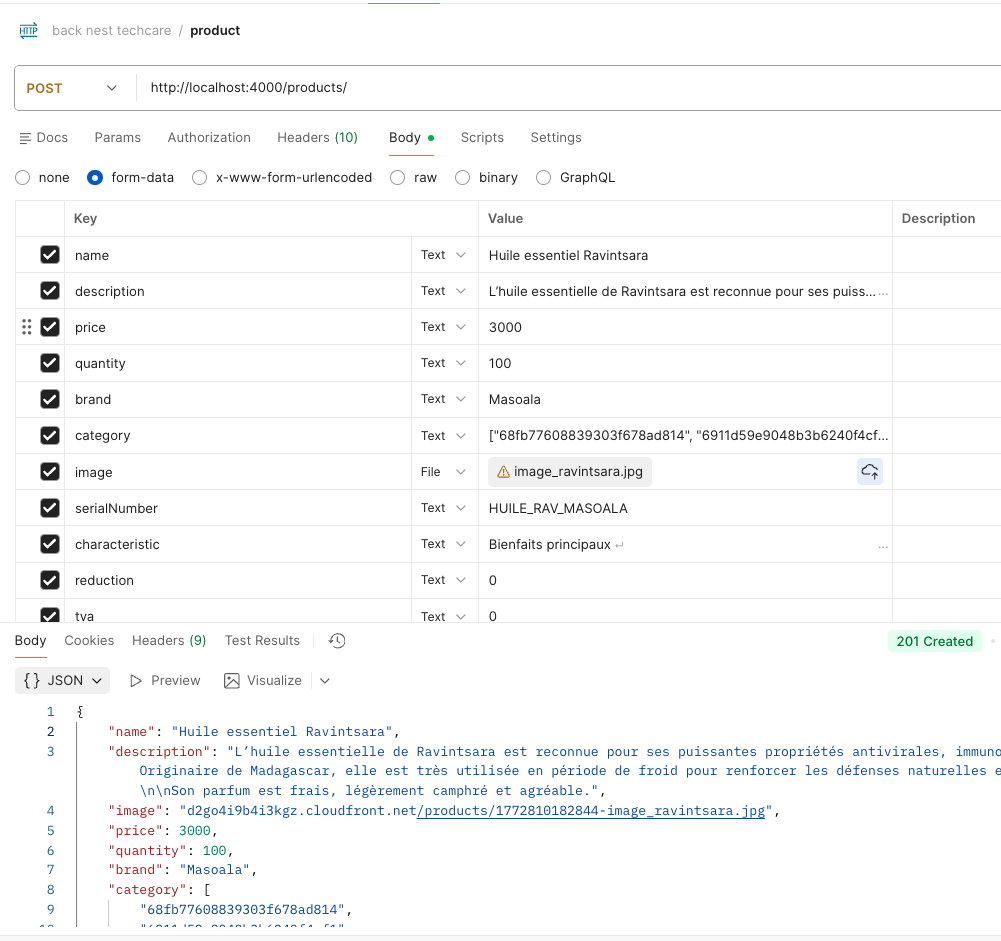
\includegraphics[width=0.9\textwidth]{postman_screenshot/product-creation-screenshot.png}
    \caption{Capture d'écran Postman : Création réussie d'un produit (201 Created)}\label{fig:postman-creation}
    \vspace{0.2cm}\small\textit{Source : Auteur}
\end{figure}

Le succès de l'opération côté client (statut \textbf{201 Created}) est quasi immédiat car le système ne bloque pas en attendant que tous les services secondaires (notifications, statistiques) aient traité l'information. En coulisses, le broker de messages prend le relais pour diffuser l'événement aux abonnés concernés.

La figure suivante montre l'activité sur l'interface d'administration de RabbitMQ au moment de la création. On y voit clairement le pic de production de messages dans la file d'attente dédiée, validant la bonne transmission de l'événement.

\begin{figure}[htbp]
    \centering
    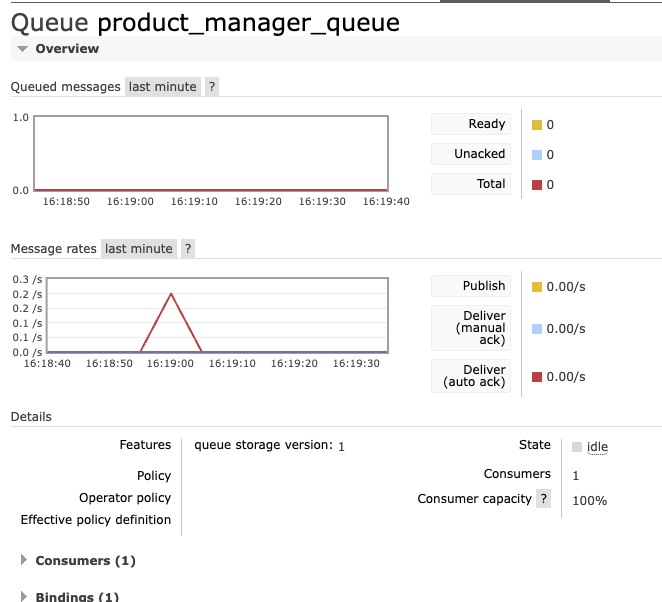
\includegraphics[width=0.9\textwidth]{postman_screenshot/event-trigger-screenshot.png}
    \caption{Interface RabbitMQ : Pic d'activité sur la file product\_manager\_queue}\label{fig:rabbitmq-event}
    \vspace{0.2cm}\small\textit{Source : Auteur}
\end{figure}

Cette approche garantit une cohérence éventuelle sur l'ensemble de la plateforme (mise à jour des notifications, synchronisation des caches, reporting) sans dégrader le temps de réponse perçu par l'utilisateur.

\subsection{IV.4.5 Validation des données et robustesse (Shared Library)}
Enfin, l'utilisation de la bibliothèque partagée (\textit{Shared Library}) permet d'unifier la validation des données grâce aux DTOs. En tentant d'envoyer des données mal formatées, le système rejette immédiatement la requête avec un message explicite.

\begin{figure}[htbp]
    \centering
    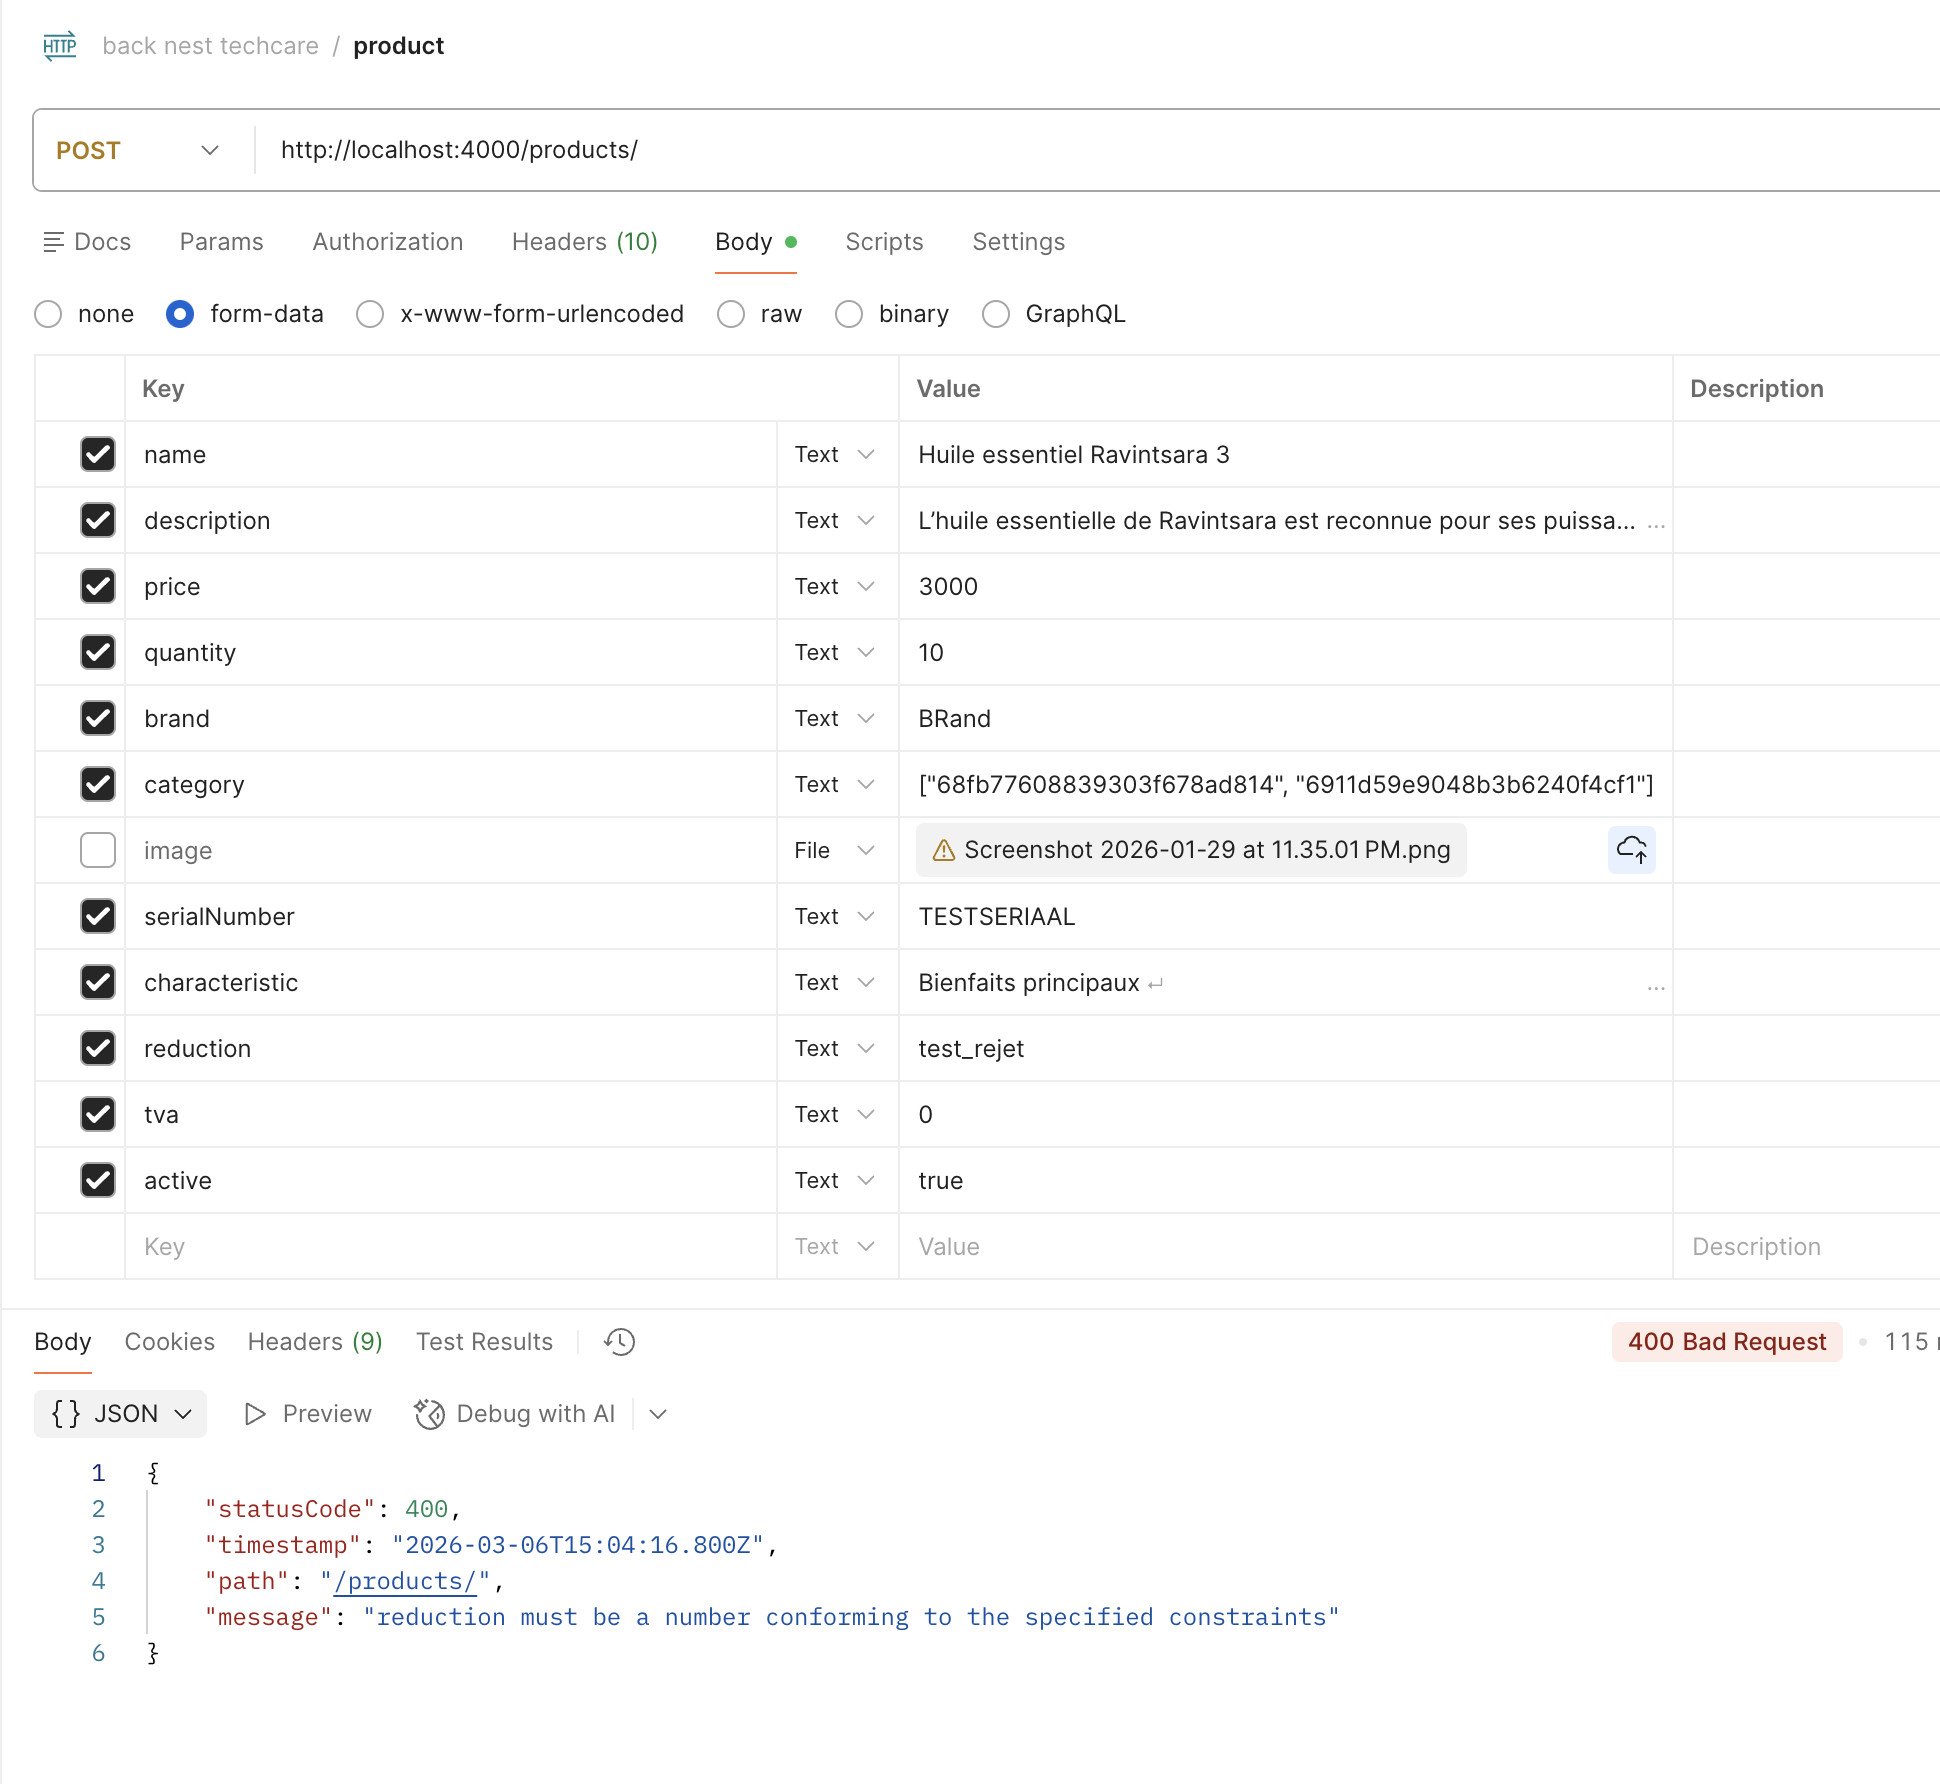
\includegraphics[width=0.9\textwidth]{postman_screenshot/validation-error-screenshot.png}
    \caption{Capture d'écran Postman : Rejet d'une requête mal formée (400 Bad Request)}\label{fig:postman-validation}
    \vspace{0.2cm}\small\textit{Source : Auteur}
\end{figure}

Comme l'illustre la capture ci-dessus, nous avons volontairement inséré une chaîne de caractères (\texttt{"test\_rejet"}) dans le champ \texttt{reduction}, qui attend spécifiquement une valeur numérique. Ce mécanisme garantit qu'aucune donnée invalide ne circule entre les microservices, renforçant la stabilité globale et simplifiant le debugging côté frontend.

\subsection{IV.4.6 Gestion des fichiers et stockage S3 (File Service)}
Lors de la création d'un produit depuis l'interface client, l'image associée (envoyée sous forme de \texttt{multipart/form-data}) est prise en charge par l'API Gateway. Avant de déclencher la création du produit en base de données, la Gateway délègue la sauvegarde de ce fichier au \textit{File Service}, qui se charge de l'uploader de manière sécurisée vers un stockage objet compatible S3 (AWS ou équivalent).

La figure ci-dessous montre la réussite de cet upload depuis l'interface de gestion S3. L'image du produit est correctement stockée et une URL publique (ou pré-signée) est générée, allégeant ainsi la base de données MongoDB qui ne conserve qu'un lien texte vers l'objet.

\begin{figure}[htbp]
    \centering
    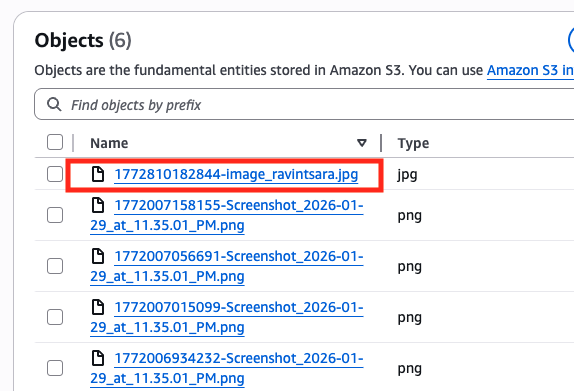
\includegraphics[width=0.8\textwidth]{postman_screenshot/s3-bucket-screenshot.png}
    \caption{Interface S3 : Validation de l'upload de l'image du produit}\label{fig:s3-upload}
    \vspace{0.2cm}\small\textit{Source : Auteur}
\end{figure}

Cette externalisation du stockage physique garantit de meilleures performances d'affichage côté client en exploitant les capacités de diffusion d'un système de fichiers distribué.
\newpage
\section{IV.5 Perspectives d'évolutions et améliorations futures}
Ce projet constitue une première étape solide qui ouvre la voie à de nombreuses optimisations.

\subsection{IV.5.1 Orchestration avec Kubernetes}
La prochaine étape logique serait la migration vers Kubernetes (K8s). Cela permettrait une auto-scalabilité dynamique des pods, une gestion plus fine des secrets et une meilleure résilience grâce au \textit{Self-healing} (redémarrage automatique des conteneurs défaillants).

\subsection{IV.5.2 Mise en place d'un Service Mesh}
Pour résoudre la complexité du traçage et de la sécurité inter-services, l'adoption d'un Service Mesh (ex: Istio) permettrait d'automatiser le chiffrement TLS entre services (mtls) et de bénéficier de tableaux de bord de monitoring avancés sans modifier le code applicatif.

\subsection{IV.5.3 CI/CD avancée}
L'automatisation complète des tests et du déploiement via GitHub Actions ou GitLab CI renforcerait encore la rapidité de livraison de Techcare, en garantissant que chaque microservice est testé isolément avant sa mise en production.

\subsection{IV.5.4 Optimisation des temps de réponse (Cache Redis)}
Pour pallier le léger ralentissement observé lors des requêtes synchrones ("impôt de la distribution"), l'ajout d'une couche de cache en mémoire avec \textbf{Redis} au niveau de l'API Gateway serait une évolution majeure. Ainsi, lors des lectures fréquentes du catalogue, la Gateway pourrait renvoyer les données quasi instantanément (2 à 5 ms) sans solliciter le \textit{Product Service} ni traverser le réseau.

\subsection{IV.5.5 Transition vers gRPC pour les communications synchrones}
Actuellement, les lectures inter-services transitent par des protocoles introduisant un surcoût de sérialisation textuelle (JSON). L'adoption de \textbf{gRPC} (Google Remote Procedure Call) pour ces échanges synchrones réduirait considérablement la taille des paquets grâce au format binaire Protobuf, et accélérerait la communication réseau.

\subsection{IV.5.6 Résilience sous haute charge : Circuit Breaking et Auto-scaling}
Les tests de stress ayant révélé des timeouts lors de pics d'activité, une perspective majeure réside dans l'implémentation de \textbf{Circuit Breakers} (via des bibliothèques comme \textit{Opossum} ou via un Service Mesh). Cela permettrait de "couper" proprement les appels vers un service saturé au lieu de laisser les requêtes s'accumuler et consommer des ressources inutilement. Couplée à l'auto-scaling horizontal des pods, cette stratégie garantirait une disponibilité de 100\% même lors de sollicitations imprévues.
\section*{Conclusion partielle}
Ce chapitre a démontré que les objectifs initiaux de scalabilité, de sécurité et de disponibilité ont été atteints. Les tests fonctionnels via Postman confirment la fiabilité des mécanismes de protection et l'efficacité des échanges asynchrones via le broker de messages. Si l'architecture microservices apporte une complexité technique supplémentaire, les bénéfices en termes d'agilité et de résilience justifient largement cet investissement pour l'évolution de la plateforme Techcare.
